% Imporditud: tools/import_eksperimendid.py
% Allikas: Eesti füüsikaolümpiaadi eksperimendi ülesannete
%   kogu (Rael Kalda, 2023), ülesanne Ü154, lahendus L154.
\setAuthor{Eero Uustalu}
\setRound{lõppvoor}
\setYear{2019}
\setNumber{G E2}
\setDifficulty{4}
\setTopic{elektriahelad}
\setVahendid{kolme väljundjuhtmega (sinine, must ja valge juhe) ``must kast'', multimeeter}
\setPunktid{14}
\setAllikas{Eksperimendi kogu Ü154, lahendus lk 113}
\setLahendusseis{toores}

\prob{Must kast}
Joonisel kujutatud kolme väljundjuhtmega ``must kast'' koosneb kolmest takistist $R_1$ , $R_2$ ja $R_3$ ning pingeallikast elektromotoorjõuga E. Määrake võimalikult täpselt $R_1$ , $R_2$ , $R_3$ ning E väärtused.
\begin{center}
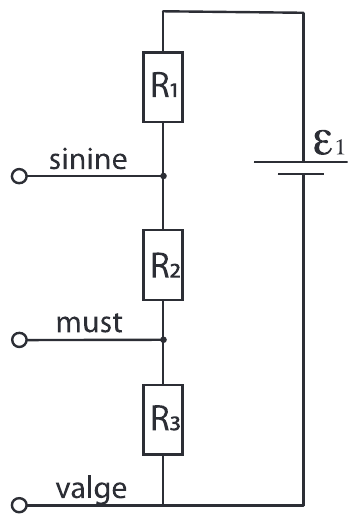
\includegraphics[width=0.28\linewidth]{2019-v3g-ge2-yl.png}
\end{center}

\hint

\solu
Ühendame ``must kasti'' musta ja valge juhtme vahele voltmeetri. Registreerime pinge $U_3$ .

$U_3$ = E (1)

$R_3$ $R_1$ + $R_2$ + $R_3$

Seejärel ühendame ``must kasti'' sinise ja valge juhtme vahele milliampermeetri (täpsem mikroampermeetri) ja mõõdame vastava voolu $I_1$:

E (2) $I_1$ = $R_1$

Seejärel ühendame ``must kasti'' musta ja valge juhtme vahele milliampermeetri (veel täpsem mikroampermeetri) ja mõõdame vastava voolu $I_2$:

E (3) $I_2$ = $R_1$ + $R_2$

Seejärel ühendame ``must kasti'' sinise ja musta juhtme vahele milliampermeetri (veel täpsem mikroampermeetri) ja mõõdame vastava voolu $I_3$:

E (4) $I_3$ = $R_1$ + $R_3$

Avaldame me valemites (2) , (3) ja (4) elektromotoorjõu E . Ühendades valemid (2) ja (3) saame avaldise:

I1R1 = I2R1 + I2R2 kust omakoda saame avaldada $R_2$ takisti $R_1$ kaudu

$R_2$ = $I_1$ $-$ $I_2$ $R_1$ (5) $I_2$

Ühendades aga valemid (2) ja (4) saame avaldise:

I1R1 = I3R1 + I3R2 kust omakoda saame avaldada $R_3$ takisti $R_1$ kaudu

$R_3$ = $I_1$ $-$ $I_3$ $R_1$ (6) $I_3$

Asetades saadud väätrused teisendatud valemisse (1) saame E väärtuse

() ( ) $I_1$ $-$$I_2$ $I_1$ $-$$I_3$ E = $U_3$ $R_1$ + $R_1$ + $R_1$ $I_3$ $\Rightarrow$ $I_2$( ) $I_1$ $-$$I_3$ $R_1$ $I_3$

( ) ( ) $I_1$ $-$$I_2$ $I_1$ $-$$I_3$ 1+ + $I_3$ E = $U_3$ I(2 ) $I_1$ $-$$I_3$

$I_3$

Edasi leiame valemitest (5) ja (6) väärtused $R_2$ ja $R_3$ ning kasutades valemit (2)

arvutame $R_1$ :

$R_1$ = E $I_1$

Kontrollkatses voltmeetri ja milliampermeetriga mõõdetud väärtused on järgmised: $U_3$ = 3,405 V $I_1$ = 1,26 mA $I_2$ = 1,022 mA $I_3$ = 0,699 mA

ja sellest tulenevad vastused: $E_1$ = 9,220 V $R_1$ = 7317 $\Omega$ $R_2$ = 1463 $\Omega$ $R_2$ = 5142 $\Omega$

Kui aga mõõta voltmeetri ja mikroampermeetriga, siis:

$U_3$ = 3,405 V $I_1$ = 1,232 mA $I_2$ = 1,022 mA $I_3$ = 0,699 mA ja sellest tulenevad vastused:

$E_1$ = 8,788 V $R_1$ = 7133 $\Omega$ $R_2$ = 1465 $\Omega$ $R_2$ = 5439 $\Omega$

Ülaltoodud vastuste erinevus tuleneb mikoampermeetri suurest ( meie takistitega lähedases suurusjärgus ) sisetakistuses mida aga kahjuks pole mõõteriista passis märgitud.
\probend
